%%%%%%%%%%%%%%%%%%%%%%%%%%%%%%%%%%%%%%%%%
% Beamer Presentation
% LaTeX Template
% Version 1.0 (10/11/12)
%
% This template has been downloaded from:
% http://www.LaTeXTemplates.com
%
% License:
% CC BY-NC-SA 3.0 (http://creativecommons.org/licenses/by-nc-sa/3.0/)
%
%%%%%%%%%%%%%%%%%%%%%%%%%%%%%%%%%%%%%%%%%

%----------------------------------------------------------------------------------------
%	PACKAGES AND THEMES
%----------------------------------------------------------------------------------------

\documentclass{beamer}

\mode<presentation> {

% The Beamer class comes with a number of default slide themes
% which change the colors and layouts of slides. Below this is a list
% of all the themes, uncomment each in turn to see what they look like.

%\usetheme{default}
%\usetheme{AnnArbor}
%\usetheme{Antibes}
%\usetheme{Bergen}
%\usetheme{Berkeley}
%\usetheme{Berlin}
%\usetheme{Boadilla}
%\usetheme{CambridgeUS}
%\usetheme{Copenhagen}
%\usetheme{Darmstadt}
%\usetheme{Dresden}
%\usetheme{Frankfurt}
%\usetheme{Goettingen}
%\usetheme{Hannover}
%\usetheme{Ilmenau}
%\usetheme{JuanLesPins}
%\usetheme{Luebeck}
\usetheme{Madrid}
%\usetheme{Malmoe}
%\usetheme{Marburg}
%\usetheme{Montpellier}
%\usetheme{PaloAlto}
%\usetheme{Pittsburgh}
%\usetheme{Rochester}
%\usetheme{Singapore}
%\usetheme{Szeged}
%\usetheme{Warsaw}

% As well as themes, the Beamer class has a number of color themes
% for any slide theme. Uncomment each of these in turn to see how it
% changes the colors of your current slide theme.

%\usecolortheme{albatross}
%\usecolortheme{beaver}
%\usecolortheme{beetle}
%\usecolortheme{crane}
%\usecolortheme{dolphin}
%\usecolortheme{dove}
%\usecolortheme{fly}
%\usecolortheme{lily}
%\usecolortheme{orchid}
%\usecolortheme{rose}
%\usecolortheme{seagull}
%\usecolortheme{seahorse}
%\usecolortheme{whale}
%\usecolortheme{wolverine}

%\setbeamertemplate{footline} % To remove the footer line in all slides uncomment this line
%\setbeamertemplate{footline}[page number] % To replace the footer line in all slides with a simple slide count uncomment this line

%\setbeamertemplate{navigation symbols}{} % To remove the navigation symbols from the bottom of all slides uncomment this line
}

\usepackage{graphicx} % Allows including images
\usepackage{booktabs} % Allows the use of \toprule, \midrule and \bottomrule in tables

%----------------------------------------------------------------------------------------
%	TITLE PAGE
%----------------------------------------------------------------------------------------

\title[ ]{MHD Simulations of Jets with Applications to the Sun} % The short title appears at the bottom of every slide, the full title is only on the title page

\author[Fionnlagh Mackenzie Dover]{Fionnlagh Mackenzie Dover \\ Supervisor: Prof R\'{o}bert Erd\'{e}lyi } % Your name
\institute[SP$^2$RC] % Your institution as it will appear on the bottom of every slide, may be shorthand to save space
{
University of Sheffield \\ % Your institution for the title page
\medskip
}
\date{03/11/2017} % Date, can be changed to a custom date

\begin{document}

\begin{frame}
\titlepage % Print the title page as the first slide
\end{frame}

\begin{frame}{Overview}

\tableofcontents % Throughout your presentation, if you choose to use \section{} and \subsection{} commands, these will automatically be printed on this slide as an overview of your presentation
\end{frame}

%----------------------------------------------------------------------------------------
%	PRESENTATION SLIDES
%----------------------------------------------------------------------------------------

%------------------------------------------------
\section{Introduction} % Sections can be created in order to organize your presentation into discrete blocks, all sections and subsections are automatically printed in the table of contents as an overview of the talk
%------------------------------------------------
\subsection{Coronal Heating} % This slide maybe a bit too basic for audience.
\begin{frame}
\begin{block}{Coronal Heating}
\begin{itemize}
\item From the core of the sun to the photosphere the temperature decreases.
\item Corona is 200 times hotter than the Sun's photosphere.
\item This contradiction is referred to as the coronal heating problem. 
\item One of the main candidates for heating the solar corona is through wave heating.
\end{itemize}
\end{block}
\begin{figure}
\centering
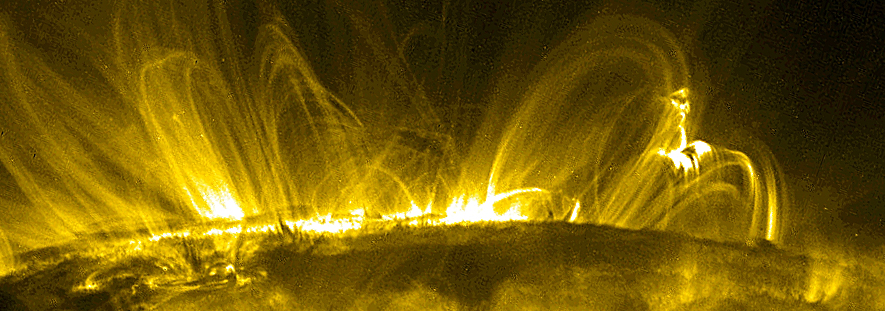
\includegraphics[width = 0.825\textwidth]{images/loop.png}
\end{figure}
\end{frame}
%----------------------------------------
\subsection{Solar Jets}
\begin{frame}{Solar Jets}
\begin{itemize}
\item give overview.
\end{itemize}
\end{frame}
%-------------------------------------------
\subsection{Transition Region Quakes} % A subsection can be created just before a set of slides with a common theme to further break down your presentation into chunks
\begin{frame}
\begin{block}{TRQ}
\begin{itemize}
\item Explain the what it is
\item Include images from scullions thesis
\end{itemize}
\end{block}
\end{frame}
\subsection{Scientific Goal}
\begin{frame}{Scientific Goal}
\begin{itemize}
\item Clearly state the problem you are investigating
\item Why should they care or what the use in it?
\end{itemize}
\end{frame}
\section{MPI-AMRVAC}
\subsection{Overview}
\begin{frame}
\begin{block}{History}
\begin{itemize}
\item VAC was developed as a flexible software focused on implementing shock capturing numerical schemes (e.g. FCT, TVD, ect). 
%\item MPI (Message Passing Interface)-AMR (Adaptive Mesh Refinement) VAC (Versatile Advection Code). 
\item Aimed at solving, primarily hyperbolic partial differential equations.  
\item MPI-AMRVAC is a parallel open source code (On Github: https://github.com/amrvac/amrvac).   
\item Written in Fortran using a pre-processor which allows to program in any dimensional matter ( LASY-syntax).  
\end{itemize}
\end{block}
\end{frame}
%------------------------------------------
\subsection{Adavitive Mesh Refienment}
\begin{frame}
\begin{block}{AMR}
\begin{itemize}
\item Block based refinement strategy used. 
\end{itemize}
\end{block}
\begin{figure}
\centering
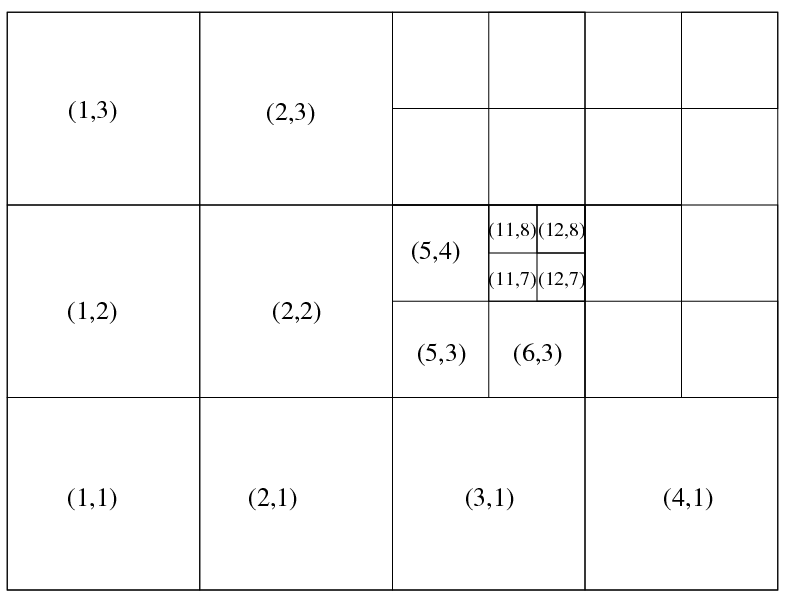
\includegraphics[width=0.5\linewidth]{images/AMR_grid.png}
\caption{Describe}
\end{figure}
\end{frame}
%-------------------------------------------------------
\begin{frame}
\begin{block}{Examples of Results of Using AMR}
\begin{itemize}
\item \href{movies/AMR_example_2.avi}{Example of AMR with 4 levels.}
\item \href{movies/tracer_jet_g.avi}{Example of HD supersonic jet with gravity acting agiant the direction of flow.}
\item \href{movies/mov_one.avi}{Example of Rayleigh Taylor simulation.}
\end{itemize}
\end{block}
\end{frame}
%---------------------------------
\begin{frame}
\begin{block}{Why use AMR}
Uniform Mesh:
\begin{itemize}
\item High resolution required for handling difficult regions (discontinuities, steep gradients, shocks, ect).
\end{itemize}
Adaptive Mesh Refinement:
\begin{itemize}
\item Start with a course grid.
\item Identify regions that need finer resolution.
\item Superimpose finer sub-grids only those regions.
\item Increased computational saving over a static grid approach. 
%\item Increased storage savings over static grid approach. 
%????? Ask Robertus about length scales involved????
\item  Track features much smaller than overall scale of the problem providing adequate higher spatial and temporal resolution where needed.    
\end{itemize}
\end{block}
\begin{figure}
\centering

\includegraphics[width=\linewidth]{images/MHD_jet.png}
\end{figure}
\end{frame}
%-------------------------------
\begin{frame}
\begin{block}{Local Error Estimation}
Outline AMR criteria.
\end{block}
\end{frame}
\subsection{MHD Module}
\begin{frame}
\begin{block}{MHD Module}
\begin{equation}
\partial_t \rho + \nabla \cdot ( \mathbf{v} \rho ) = 0
\end{equation}
\begin{equation}
\partial_t (\rho \mathbf{v})+ \nabla \cdot (\mathbf{v} \rho \mathbf{v} - \mathbf{BB}) + \nabla p_{tot} = 0 ,
\end{equation}
\begin{equation}
\partial_t e + \nabla \cdot (\mathbf{v} e - \mathbf{BB} \cdot \mathbf{v}+\mathbf{v} p_{tot}) = \nabla \cdot (\mathbf{B} \times \eta \mathbf{J} ) ,
\end{equation}
\begin{equation}
\partial_t \mathbf{B} + \nabla \cdot (\mathbf{vB}-\mathbf{Bv}) = - \nabla \times (\eta \mathbf{J}) .
\end{equation}
Where:
\begin{equation}
p = (\gamma -1) \left( e -  \frac{\rho \mathbf{v}^2}{2} - \frac{\mathbf{B}^2}{2} \right) ,
\end{equation}
\begin{equation}
p_{tot} = p + \frac{\mathbf{B}^2}{2}, \ \ \ \mathbf{J} = \nabla \times \mathbf{B}. 
\end{equation}
\begin{itemize}
\item Explain why the equations are in this conservative form. 
\item Explain the addition of source terms (i.e. gravity). 
\end{itemize}
\end{block}
\end{frame}
%------------------------------------------------
\section{Jet Simulations}
\subsection{Set up}
\begin{frame}
\begin{block}{Set up}
\begin{itemize}
\item Show line plots of profiles used. Compare against VALC data (see Ronnie PhD student thesis plots).
\item Explain the BC conditions you are using.
\item Video of the background being stable. 
\item Explain the driver of the jet.
\end{itemize}
\end{block}
\end{frame}
\subsection{Results}
\begin{frame}
\begin{block}{Results}
MOVIES
\end{block}
\end{frame}
\section{Conclusion and Future Plans}
\begin{frame}
\begin{block}{Conclusion}

\end{block}
\end{frame}
%----------------------------------
\begin{frame}
\begin{block}{Future Plans}

\end{block}
\end{frame}

%----------------------------------------------------------------------------------------

\end{document}
